\documentclass[answers]{exam}
\usepackage[english]{babel}
\usepackage[utf8x]{inputenc}
\usepackage{amsmath,amssymb,amsthm}

\usepackage[table,dvipsnames]{xcolor}
\usepackage{graphicx}
\usepackage{pgf,tikz,tikz-3dplot}
\usetikzlibrary{shapes,arrows,positioning,backgrounds}
\tikzset{%
	roundnode/.style={circle, draw=MidnightBlue!90, thick, fill=gray!40},
	pt/.style={draw=MidnightBlue, thick,->,>=stealth',shorten >=1pt},
	fwd/.style={preaction={draw=YellowOrange,-, line width=2pt,shorten >=3pt}}
}
\usepackage{float}

\begin{document}

\noindent{\large OPER 640 - Stochastic Modeling and Analysis I%
	% Homework X % (Due Jan X at 10am)
	}
\hspace{\fill} {\large B. Hosley}
\bigskip

\begin{questions}

%%%%%%%%%%%%%%%%%%%%%%%%%%%
%	\begin{ Question 1}	  %
%%%%%%%%%%%%%%%%%%%%%%%%%%%
\question 
\emph{Modeling Exercise 2.6 (page 44). Specify both the transition matrix and the transition diagram.}

A machine consists of $K$ components in series,i.e.,all the components must be in working condition for the machine to be functional. When the machine is functional at the beginning of the nth day, each component has a probability $p$ of failing at the beginning of the next day, independent of the other components. (More than one component can fail at the same time.) When the machine fails, a single repair person repairs the failed components one by one. It takes exactly one day to repair one failed component. When all the failed components are repaired the machine is functional again, and behaves as before. When the machine is down, the working components do not fail. Let \(X_n\) be the number of failed components at the beginning of the $n$th day, after all the failure and repair events at that time are accounted for.

Show that \({X_n,n ≥ 0}\) is a DTMC. Display its transition matrix or the transition diagram.
\begin{solution}
	Where the nodes represent the number of broken components:
	
\begin{figure}[H]
	\centering
	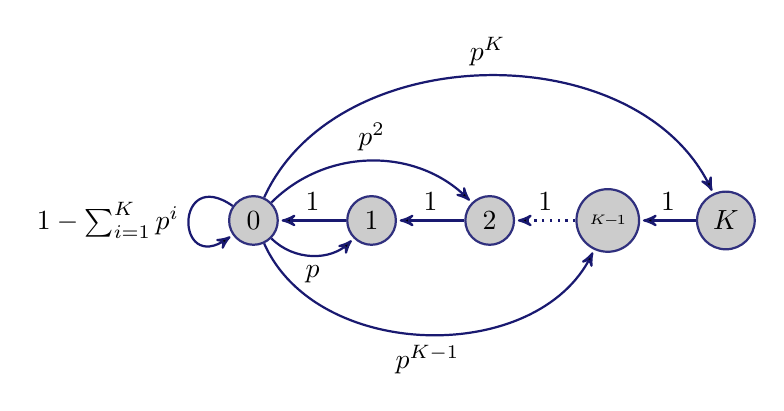
\begin{tikzpicture}[node distance=1.5cm]		
		\node[roundnode] (zero) {0};
		\node[roundnode] (one) [right of=zero] {1};
		\node[roundnode] (two) [right of=one] {2};
		\node[roundnode] (three) [right of=two] {\tiny $K\!\!-\!\!1$};
		\node[roundnode] (four) [right of=three] {$K$};
		
		\path[pt] (one) 	edge []  node [above] 	{1} (zero);
		\path[pt] (two) 	edge []  node [above] 	{1} (one);
		\path[pt] (four) 	edge []  node [above] 	{1} (three);
		\path[pt] (three) 	edge [dotted]  node [above] 	{1} (two);
		
		\path[pt] (zero)	edge [bend right=45]	node [below]	{$p$} (one);
		\path[pt] (zero) 	edge [bend left=45]		node [above]	{$p^2$} (two);
		\path[pt] (zero)	edge [bend right=65]	node [below]	{$p^{K-1}$} (three);
		\path[pt] (zero) 	edge [bend left=65]		node [above]	{$p^K$} (four);
		
		\path[pt] (zero) 	edge [loop left, min distance=9mm, out=145, in=215]	node [left]	{$1-\sum_{i=1}^{K}p^i$} (zero);
	\end{tikzpicture}
	\caption{}
\end{figure}

\begin{align*}
	P =
	\begin{bmatrix}
		1-\sum_{i=1}^{K}p^i & p & p^2 & \cdots & p^{K-1} & p^K \\
		1 & 0 & 0 & \cdots & 0 & 0 \\
		0 & 1 & 0 & \cdots & 0 & 0 \\
		0 & 0 & 1 & \cdots & 0 & 0 \\
		\vdots & \vdots & \vdots & \ddots & \vdots & \vdots \\
		0 & 0 & 0 & \cdots & 0 & 0 \\
		0 & 0 & 0 & \cdots & 1 & 0 \\
	\end{bmatrix}
\end{align*}


\end{solution}
%\end{ Question 1}

%%%%%%%%%%%%%%%%%%%%%%%%%%%
%	\begin{ Question 2}	  %
%%%%%%%%%%%%%%%%%%%%%%%%%%%
\question 
\emph{Modeling Exercise 2.8 (page 45). Specify both the transition matrix and the transition diagram.}

Consider the following weather forecasting model:if today is sunny(rainy)and it is the k-th day of the current sunny (rainy) spell, then it will be sunny (rainy) tomorrow with probability \(p_k (q_k)\) regardless of what happened before the current sunny (rainy) spell started (k ≥ 1). Model this as a DTMC. What is the state-space? What are the transition probabilities?
\begin{solution}
	
	The state space is Sunny (S) and Rainy (R).
	
	\(S=\{\text{S,R}\}\)
	
\begin{figure}[H]
	\centering
	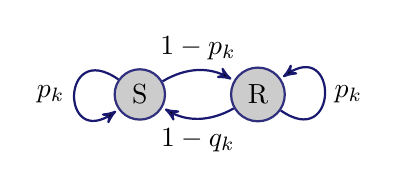
\begin{tikzpicture}[node distance=1.5cm]		
		\node[roundnode] (zero) {S};
		\node[roundnode] (one) [right of=zero] {R};	
		
		\path[pt] (zero)	edge [bend left]	node [above]	{$1-p_k$} (one);
		\path[pt] (one) 	edge [bend left]	node [below]	{$1-q_k$} (zero);
		
		\path[pt] (zero) 	edge [loop left, min distance=9mm, out=145, in=215]	node [left]	{$p_k$} (zero);
		\path[pt] (one) 	edge [loop right, min distance=9mm, out=-35, in=35]	node [right]	{$p_k$} (one);
	\end{tikzpicture}
	\caption{}
\end{figure}

Where Sunny is the $0^{th}$ index and Rainy is $1$.
\begin{align*}
	P =
	\begin{bmatrix}
		p_k & 1-p_k \\
		1-q_k & q_k \\
	\end{bmatrix}
\end{align*}
	
\end{solution}
%\end{ Question 2}

%%%%%%%%%%%%%%%%%%%%%%%%%%%
%	\begin{ Question 3}	  %
%%%%%%%%%%%%%%%%%%%%%%%%%%%
\question 
\emph{Modeling Exercise 2.14 (page 46). Also specify the transition diagram.}

A machine with two components is subject to a series of shocks that occur deterministically one per day. When the machine is working a shock can cause failure of component 1 alone with probability \(\alpha_1\), or of component 2 alone with probability \(\alpha_2\) or of both the components with probability \(\alpha_{12}\) or no failures with probability \(\alpha_0\). (Obviously $\alpha_0+\alpha_1+\alpha_2+\alpha_{12} =1$.)When a failure occurs,the machine is shutdown and no more failures occur until the machine is repaired. The repair time (in days) of component $i (i = 1, 2)$ is a geometric random variable with parameter $r_i , 0 < r_i < 1$. Assume that there is a single repair person and all repair times are independent. If both components fail simultaneously, the repair person repairs component one first, followed by component two. Give the state-space and the transition probability matrix of an appropriate DTMC that can be used to model the state-evolution of the machine.
\begin{solution}
	
	\begin{figure}[H]
		\centering
		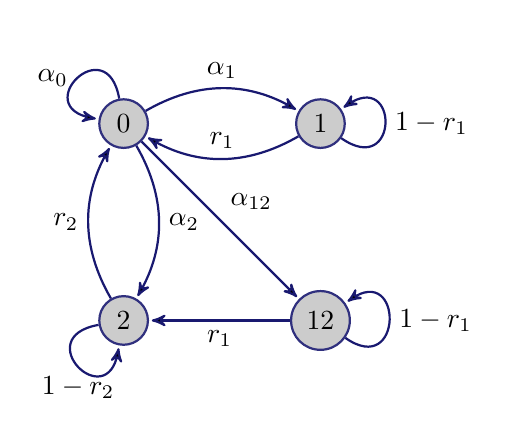
\begin{tikzpicture}[node distance=2.5cm]	
			\node[roundnode] (zero) {0};
			\node[roundnode] (one) [right of=zero] {1};	
			\node[roundnode] (two) [below of=zero] {2};
			\node[roundnode] (three) [right of=two] {12};
				
			\path[pt] (zero) 	edge [loop left, min distance=9mm, out=100, in=170]	node [left]	{$\alpha_0$} (zero);
			\path[pt] (zero)	edge [bend left]	node [above]	{$\alpha_1$} (one);
			\path[pt] (zero)	edge [bend left]	node [right]	{$\alpha_2$} (two);
			\path[pt] (zero)	edge []				node [above right]	{$\alpha_{12}$} (three);
			
			\path[pt] (one) 	edge [loop right, min distance=9mm, out=-35, in=35]	node [right]	{$1-r_1$} (one);
			\path[pt] (one) 	edge [bend left]	node [above]	{$r_1$} (zero);
			
			\path[pt] (two) 	edge [loop right, min distance=9mm, out=-170, in=-100]	node [below]	{$1-r_2$} (two);
			\path[pt] (two) 	edge [bend left]	node [left]	{$r_2$} (zero);
			
			\path[pt] (three) 	edge [loop right, min distance=9mm, out=-35, in=35]	node [right]	{$1-r_1$} (three);
			\path[pt] (three) 	edge []	node [below]	{$r_1$} (two);
			
		\end{tikzpicture}
		\caption{}
	\end{figure}
\end{solution}
%\end{ Question 3}

%%%%%%%%%%%%%%%%%%%%%%%%%%%
%	\begin{ Question 4}	  %
%%%%%%%%%%%%%%%%%%%%%%%%%%%
\question 
Q
\begin{solution}
	S
\end{solution}
%\end{ Question 4}

%%%%%%%%%%%%%%%%%%%%%%%%%%%
%	\begin{ Question 5}	  %
%%%%%%%%%%%%%%%%%%%%%%%%%%%
\question 
Q
\begin{solution}
	S
\end{solution}
%\end{ Question 5}

%%%%%%%%%%%%%%%%%%%%%%%%%%%
%	\begin{ Question 6}	  %
%%%%%%%%%%%%%%%%%%%%%%%%%%%
\question 
Q
\begin{solution}
	S
\end{solution}
%\end{ Question 6}

%%%%%%%%%%%%%%%%%%%%%%%%%%%
%	\begin{ Question 7}	  %
%%%%%%%%%%%%%%%%%%%%%%%%%%%
\question 
Q
\begin{solution}
	S
\end{solution}
%\end{ Question 7}

%%%%%%%%%%%%%%%%%%%%%%%%%%%
%	\begin{ Question 8}	  %
%%%%%%%%%%%%%%%%%%%%%%%%%%%
\question 
Q
\begin{solution}
	S
\end{solution}
%\end{ Question 8}

%%%%%%%%%%%%%%%%%%%%%%%%%%%
%	\begin{ Question 9}	  %
%%%%%%%%%%%%%%%%%%%%%%%%%%%
\question 
Q
\begin{solution}
	S
\end{solution}
%\end{ Question 9}

%%%%%%%%%%%%%%%%%%%%%%%%%%%
%  \begin{ Question 10}	  %
%%%%%%%%%%%%%%%%%%%%%%%%%%%
\question 
Q
\begin{solution}
	S
\end{solution}
%\end{ Question 10}

\end{questions}
\end{document}